\newpage
\titledquestion{Filling in the Blanks}

\textbf{Filling in the Blanks}

Recall the notion of an \textit{optree}, which is a tree that corresponds to an
arithmetic expression, where the nodes are operators and the leaves are integers.

Unfortunately, a dog has eaten all of our operators!

A \textit{skeleton} is an optree whose operators are missing:

\begin{codeblock}
  datatype skel = Leaf of int | Blank of skel * skel

  datatype oper = Plus | Minus
  datatype expr = Val of int | Node of expr * oper * expr

  fun evalExpr (Val n) = n
    | evalExpr (Node (l, Plus,  r)) = evalExpr l + evalExpr r
    | evalExpr (Node (l, Minus, r)) = evalExpr l - evalExpr r
\end{codeblock}

Our goal will be to take a \code{skel} and fill in each \code{Blank} node to obtain
an \code{expr}. Each \code{Blank} may become either \code{Plus} or \code{Minus},
so a skeleton with $k$ blanks has $2^k$ fillings:

\begin{center}
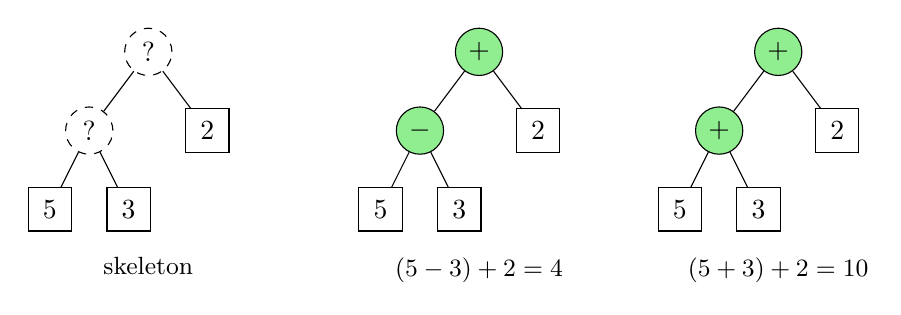
\begin{tikzpicture}[
  level 1/.style={sibling distance=15mm},
  level 2/.style={sibling distance=10mm},
  level distance=10mm,
  every node/.style={inner sep=1.5pt},
  blank/.style={circle, draw, dashed, minimum size=6mm},
  op/.style={circle, draw, fill=LightGreen, minimum size=6mm},
  lf/.style={rectangle, draw, minimum size=5.5mm},
  treecap/.style={anchor=north},          % captions share one baseline
]
%% Each tree is rooted at y=0 and is 2 levels deep, so every caption
%% hangs from the same y -- keeps the three columns visually aligned.
\def\capy{-2.55}

%% ---- skeleton ----
\begin{scope}
  \node[blank] {?}
    child {node[blank] {?}
      child {node[lf] {5}}
      child {node[lf] {3}}}
    child {node[lf] {2}};
  \node[treecap] at (0,\capy) {\small skeleton};
\end{scope}

\node at (2.35,-1.0) {\large $\rightsquigarrow$};

%% ---- filling A ----
\begin{scope}[xshift=4.2cm]
  \node[op] {$+$}
    child {node[op] {$-$}
      child {node[lf] {5}}
      child {node[lf] {3}}}
    child {node[lf] {2}};
  \node[treecap] at (0,\capy) {\small $(5-3)+2 = 4$};
\end{scope}

%% ---- filling B ----
\begin{scope}[xshift=8.0cm]
  \node[op] {$+$}
    child {node[op] {$+$}
      child {node[lf] {5}}
      child {node[lf] {3}}}
    child {node[lf] {2}};
  \node[treecap] at (0,\capy) {\small $(5+3)+2 = 10$};
\end{scope}
\end{tikzpicture}
\end{center}

\noindent
This skeleton has four fillings in all, evaluating to \code{4}, \code{10},
\code{0}, and \code{6}. Nothing fills it to \code{7}.

We search for a filling in CPS. One continuation \code{k} is offered each candidate, and returns
\code{SOME} to accept it or \code{NONE} to make \code{fill} try the next.

\begin{parts}
  \part[12]\hfill

    Implement \code{fill}:

    \spec
      {fill}
      {\code{skel -> (expr * int -> expr option) -> expr option}}
      {\code{k} is total}
      {\code{fill s k} offers \code{k} each way of filling \code{s}, as a pair
      \code{(e, v)} of a filled-in expression \code{e} and its value \code{v}.
      It returns the first \code{SOME} that \code{k} produces, or \code{NONE} if
      \code{k} rejects every filling.}

    \begin{solutionorbox}[26em]
      \begin{codeblock}
        fun fill (Leaf n) k = k (Val n, n)
          | fill (Blank (l, r)) k =
              fill l (fn (le, a) =>
                fill r (fn (re, b) =>
                  case k (Node (le, Plus, re), a + b) of
                    SOME res => SOME res
                  | NONE => k (Node (le, Minus, re), a - b)))
      \end{codeblock}

      To fill a \code{Blank}, we fill the left subtree; its continuation fills the
      right subtree; and \textit{that} continuation has both filled subtrees
      \code{le} and \code{re} in hand, so it can build the node. It offers the
      \code{Plus} version to \code{k}; only if \code{k} rejects it (\code{NONE})
      does it fall back to the \code{Minus} version.
    \end{solutionorbox}

  \part[3]\hfill

    Using \code{fill}, implement \code{solve}.

    \spec
      {solve}
      {\code{skel -> int -> expr option}}
      {\code{true}}
      {\code{solve s target} evaluates to \code{SOME e}, where \code{e} is a
      filling of \code{s} with \code{evalExpr e} $\eeq$ \code{target}, or
      \code{NONE} if no such filling exists.}

    \begin{solutionorbox}[12em]
      \begin{codeblock}
        fun solve s target =
          fill s (fn (e, v) =>
            if v = target then SOME e else NONE)
      \end{codeblock}

      The continuation is the goal test: accept a candidate (\code{SOME e}) when
      its value matches the target, and reject it (\code{NONE}) otherwise ---
      which tells \code{fill} to keep searching.
    \end{solutionorbox}

  \newpage

  \part[8]\hfill

    \code{fill} stops at the first accepted filling. Now we want all of them.
    Implement \code{fillAll}:

    \spec
      {fillAll}
      {\code{skel -> (expr * int -> 'a list) -> 'a list}}
      {\code{k} is total}
      {\code{fillAll s k} evaluates to the concatenation of \code{k (e, v)} over
      \textbf{every} filling \code{(e, v)} of \code{s}.}

    Then implement \code{solveAll} using it:

    \spec
      {solveAll}
      {\code{skel -> int -> expr list}}
      {\code{true}}
      {\code{solveAll s target} evaluates to a list of all fillings \code{e} of
      \code{s} with \code{evalExpr e} $\eeq$ \code{target}.}

    \begin{solutionorbox}[30em]
      \begin{codeblock}
        fun fillAll (Leaf n) k = k (Val n, n)
          | fillAll (Blank (l, r)) k =
              fillAll l (fn (le, a) =>
                fillAll r (fn (re, b) =>
                    k (Node (le, Plus,  re), a + b)
                  @ k (Node (le, Minus, re), a - b)))

        fun solveAll s target =
          fillAll s (fn (e, v) =>
            if v = target then [e] else [])
      \end{codeblock}

      The only change from \code{fill} is what happens at a \code{Blank}: instead
      of trying \code{Plus} and falling back to \code{Minus} only on rejection,
      we take \textbf{both} and \code{@} their results together --- so nothing is
      ever cut off. The continuation reports zero or more results per candidate
      (\code{[e]} to keep it, \code{[]} to drop it), and the concatenation
      accumulates them all.
    \end{solutionorbox}
\end{parts}
